\documentclass[a4paper, 12pt]{article}%тип документа

%отступы
\usepackage[left=2cm,right=2cm,top=2cm,bottom=3cm,bindingoffset=0cm]{geometry}
\setlength{\parindent}{5ex}

%Русский язык
\usepackage[T2A]{fontenc} %кодировка
\usepackage[utf8]{inputenc} %кодировка исходного кода
\usepackage[english,russian]{babel} %локализация и переносы

%Вставка картинок
\usepackage{graphicx}
\graphicspath{{pictures/}}
\DeclareGraphicsExtensions{.pdf,.png,.jpg}

%Графики
\usepackage{pgfplots}
\pgfplotsset{compat=1.9}

%Математика
\usepackage{amsmath, amsfonts, amssymb, amsthm, mathtools}

%Таблицы
\usepackage{longtable} 
\usepackage{float}

%Римские цифры
\newcommand{\RomanNumeralCaps}[1]{\uppercase\expandafter{\romannumeral#1}}

\usepackage{multirow}


\begin{document}
	\begin{titlepage}
		\begin{center}
			\textsc{Федеральное государственное автономное образовательное учреждение высшего образования«Московский физико-технический институт (национальный исследовательский университет)»\\[5mm]
			}
			
			\vfill
			
			\textbf{Отчёт по лабораторной работы 2.5.1\\[3mm]
				Измерение коэффициента поверхностного натяжения жидкости.
				\\[50mm]
			}
			
		\end{center}
		
		\hfill
		\begin{minipage}{.5\textwidth}
			Выполнил студент:\\[2mm]
			Сериков Василий Романович\\[2mm]
			группа: Б03-102\\[5mm]
			
		\end{minipage}
		\vfill
		\begin{center}
			Москва, 2022 г.
		\end{center}
		
	\end{titlepage}
	
	\newpage
	\textbf{Аннотация}\\
	
	
	\textbf{Цель работы: }\\
	
1) измерение температурной зависимости коэффициента поверхностного
натяжения дистиллированной воды с использованием известного коэффициента
поверхностного натяжения спирта; 2) определение полной поверхностной энергии и
теплоты, необходимой для изотермического образования единицы поверхности жидкости
при различной температуре.\\
	
	
	\textbf{Теоретические сведения: } \\

	
	Наличие поверхностного слоя приводит к различию давлений по разные стороны от искривленной границы раздела двух сред.  Для сферического пузырька с воздухом  внутри жидкости избыточное давление даётся формулой Лапласа:
	
	\begin{equation}\label{key}
		\Delta P = P_{int} - P_{ext} = \frac{2\sigma}{r},
	\end{equation}
	где $ \sigma $ -- коэффициент поверхностного натяжения, $ P_{int} $ и $ P_{ext} $ -- давление внутри пузырька и снаружи, $ r $ -- радиус кривизны поверхности раздела двух фаз. Эта формула лежит в основе предлагаемого метода определения коэффициента поверхностного натяжения жидкости. Измеряется давление $ \Delta P $, необходимое для выталкивания в жидкость пузырька воздуха.\\
	
	
\textbf{Методика измерений: }\\
	
	\begin{figure}[h]
		\center{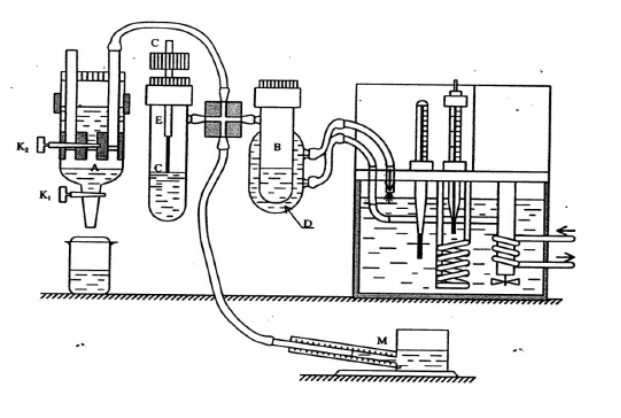
\includegraphics [scale=1]{installation.png}}
		\caption{Схема экспериментальной установки}
	\end{figure}
	
	Исследуемая жидкость (дистиллированная вода) наливается в сосуд (колбу) $ B $ (рис.1). Тестовая жидкость  (этиловый спирт) наливается  в сосуд $ E $.  При измерениях  колбы герметично закрываются  пробками. Через одну из двух пробок  проходит полая металлическая игла $ С $. Этой пробкой закрывается сосуд, в котором  проводятся измерения. Верхний конец иглы открыт в атмосферу, а нижний погружен в жидкость. Другой сосуд герметично закрывается второй пробкой. При создании достаточного  разряжения воздуха в колбе с иглой пузырьки воздуха начинают пробулькивать через жидкость. Поверхностное натяжение можно определить по величине разряжения $ \Delta P $ \eqref{key}, необходимого для прохождения пузырьков (при известном радиусе иглы).
	
	Разряжение в системе создается с помощью аспиратора $ A $. Кран $ K_2 $ разделяет две полости аспиратора. Верхняя полость при закрытом кране $ K_2 $ заполняется водой. Затем кран $ K_2 $ открывают и заполняют водой  нижнюю полость  аспиратора.  Разряжение воздуха создается в нижней полости  при открывании крана $ K_1 $, когда  вода вытекает из неё по каплям. В колбах $ В $ и $ С $, соединённых трубками с нижней полостью аспиратора, создается такое же пониженное давление. Разность давлений в полостях с разряженным воздухом и атмосферой измеряется спиртовым микроманометром. 
	
	Для стабилизации температуры исследуемой жидкости через рубашку $ D $ колбы $ В $ непрерывно прогоняется вода из термостата.
	
	Обычно кончик иглы лишь касается поверхности жидкости, чтобы исключить влияние гидростатического давления столба жидкости. Однако при измерении температурной зависимости коэффициента поверхностного натяжения возникает ряд сложностей. Во-первых, большая теплопроводность металлической трубки приводит к тому, что температура на конце трубки заметно ниже, чем в глубине жидкости. Во-вторых, тепловое расширение поднимает уровень жидкости при увеличении температуры.
	
	Обе погрешности можно устранить, погрузив кончик трубки до самого дна. Полное давление, измеренное при этом микроманометром, равно \[ P = \Delta P + \rho g h.\] Заметим, что $ \rho gh $ от температуры практически не зависит, так как подъём уровня жидкости компенсируется уменьшением её плотности (произведение $ \rho g $ определяется массой всей жидкости и поэтому постоянно). Величину  $ \rho g h $ следует измерить двумя способами.
	
	Во-первых, замерить величину $ P_1= \Delta P' $, когда кончик трубки только касается поверхности жидкости. Затем при этой же температуре опустить иглу до дна и замерить $ P_2= \rho gh + \Delta P'' $ ($ \Delta P' $, $ \Delta P'' $ -- давление Лапласа). Из-за  несжимаемости  жидкости можно положить $ \Delta P' = \Delta P'' $ и тогда \[ \rho gh= P_2 - P_1. \]
	
	Во-вторых, при измерениях $ P_1 $ и $ P_2 $ замерить линейкой  глубину погружения иглы $ h $. Это можно сделать, замеряя расстояние между верхним концом иглы и любой неподвижной частью прибора при положении иглы на поверхности и в глубине колбы.\\
	
	
	\textbf{Используемое оборудование: }\\
	
	Прибор Ребиндера с термостатом и микроманометром;
	исследуемые жидкости; стаканы.\\
	
	\newpage
	
		\textbf{Результаты измерений и обработка данных: }\\
	\begin{enumerate}
	\item Начальные данные и погрешности: $\sigma_p = \pm 0,5$мм - погрешность манометра, $\sigma_{\text{спирт}} = 0,0224$ Н/м - коэффициент поверхностного натяжения спирта при 20$^\circ C$, d = 1,15$\pm 0,05$ мм - диаметр иглы, измеренный при помощи микроскопа.
	
	
	\item Измерим максимальное давление $P$ при пробулькивании пузырьков воздуха через спирт. Пользуясь табличным значением коэффициента поверхностного натяжения спирта, определим по формуле (1) диаметр иглы. Сравним полученный результат с диаметром иглы, измеренным по микроскопу.
	
	\begin{longtable} {|c|c|c|c|}
		\hline
		№ & $ P $, мм. &  $ P $, Па  & $ \overline P  $, Па    \\ \hline
		1 & 42  & 82 & \multirow{5}{*}{$81 \pm 1$}  \\ \cline{1-3}
		2 & 41,5  & 81 &     \\ \cline{1-3}
		3 & 41,5  & 81 &     \\ \cline{1-3}
		4 & 41,5  & 81 &   \\ \hline
		\caption{Результаты измерений в спирте}
	\end{longtable}
	
	$$ d = \frac{4 \cdot \sigma_{\text{спирт}}}{P} = 1,09 \pm 0,01 \text{ мм}$$
	
	
	
	\item Измерим максимальное давление $P_1$ при пробулькивании
	пузырьков, когда игла лишь касается поверхности воды. Измерим расстояние $h_1$
	между верхним концом иглы и любой неподвижной часть прибора. Потом утопим иглу до предела, чтобы измерьте максимальное давление в пузырьках Р2 и расстояние $h_2$. По разности давлений $\Delta P = P_2 - P_1$ определим глубину погружения $\Delta h$ иглы и сравним с $\Delta h = h_1- h_2$.
	
	\begin{longtable} {|c|c|c|c|c|}
		\hline
		№ & $ P $, мм &  $ P $, Па  & $ \overline P_1  $, Па  & $h_1$, мм             \\ \hline
		1 & 98  & 192 & \multirow{5}{*}{$190 \pm 1$} &\multirow{5}{*}{$21,5 \pm 0,5$} \\ \cline{1-3}
		2 & 97  & 190 &                     &             \\ \cline{1-3}
		3 & 97  & 190 &                     &                      \\ \cline{1-3}
		4 & 96  & 188 &                     &                      \\ \hline
		\caption{Результаты измерений в воде}
	\end{longtable}
	
		\begin{longtable} {|c|c|c|c|c|}
		\hline
		№ & $ P $, мм &  $ P $, Па  & $ \overline P_2  $, Па  & $h_2$, мм             \\ \hline
		1 & 178  & 349 & \multirow{5}{*}{$349 \pm 1$} &\multirow{5}{*}{$6,5 \pm 0,5$} \\ \cline{1-3}
		2 & 178  & 349 &                     &             \\ \cline{1-3}
		3 & 178 & 349&                     &                      \\ \cline{1-3}
		4 & 178 & 349 &                     &                      \\ \hline
		\caption{Результаты измерений в воде}
	\end{longtable}
	
	
	$$ \Delta h = \frac{\overline P_2 - \overline P_1}{\rho \cdot g} = 16 \pm 1 \text{ мм}$$
	
	$$ \Delta h = h_1 - h_2 = 15 \pm 1 \text{мм} $$
	 
	
	\item Снимем температурную зависимость $\sigma (T)$ для дистиллированной воды.Для уменьшения погрешности опыта замер давления при фиксированной температуре проведем несколько раз.
	
	
	\begin{longtable} {|c|c|c|c|c|}
		\hline
		№ & $ P $, мм &  $ P $, Па  & $ \overline P  $, Па  & $T$, К             \\ \hline
		1 & 194 & 381 & \multirow{5}{*}{$381 \pm 1$} &\multirow{5}{*}{298} \\ \cline{1-3}
		2 & 193,5  & 380 &                     &             \\ \cline{1-3}
		3 & 193,5 & 380&                     &                      \\ \cline{1-3}
		4 & 194 & 381 &                     &                      \\ \hline
		\caption{Результаты измерений при Т = 298 К }
	\end{longtable}

\begin{longtable} {|c|c|c|c|c|}
	\hline
	№ & $ P $, мм &  $ P $, Па  & $ \overline P  $, Па  & $T$, К             \\ \hline
	1 & 192,5 & 378 & \multirow{5}{*}{$378 \pm 1$} &\multirow{5}{*}{303} \\ \cline{1-3}
	2 & 192,5  & 378 &                     &             \\ \cline{1-3}
	3 & 193 & 379&                     &                      \\ \cline{1-3}
	4 & 192 & 377 &                     &                      \\ \hline
	\caption{Результаты измерений при Т = 303 К }
\end{longtable}

\begin{longtable} {|c|c|c|c|c|}
	\hline
	№ & $ P $, мм &  $ P $, Па  & $ \overline P  $, Па  & $T$, К             \\ \hline
	1 & 191,5 & 376 & \multirow{5}{*}{$376 \pm 1$} &\multirow{5}{*}{308} \\ \cline{1-3}
	2 & 191,5  & 376 &                     &             \\ \cline{1-3}
	3 & 191,5 & 376 &                     &                      \\ \cline{1-3}
	4 & 191,5 & 376 &                     &                      \\ \hline
	\caption{Результаты измерений при Т = 308 К }
\end{longtable}

\begin{longtable} {|c|c|c|c|c|}
	\hline
	№ & $ P $, мм &  $ P $, Па  & $ \overline P  $, Па  & $T$, К             \\ \hline
	1 & 190 & 373 & \multirow{5}{*}{$374 \pm 1$} &\multirow{5}{*}{313} \\ \cline{1-3}
	2 & 190,5  & 374 &                     &             \\ \cline{1-3}
	3 & 190,5 & 374&                     &                      \\ \cline{1-3}
	4 & 190 & 373 &                     &                      \\ \hline
	\caption{Результаты измерений при Т = 313 К }
\end{longtable}

\begin{longtable} {|c|c|c|c|c|}
	\hline
	№ & $ P $, мм &  $ P $, Па  & $ \overline P  $, Па  & $T$, К             \\ \hline
	1 & 189 & 371 & \multirow{5}{*}{$371 \pm 1$} &\multirow{5}{*}{318} \\ \cline{1-3}
	2 & 189  & 371 &                     &             \\ \cline{1-3}
	3 & 189,5 & 372&                     &                      \\ \cline{1-3}
	4 & 189 & 371 &                     &                      \\ \hline
	\caption{Результаты измерений при Т = 318 К }
\end{longtable}

\newpage

\begin{longtable} {|c|c|c|c|c|}
	\hline
	№ & $ P $, мм &  $ P $, Па  & $ \overline P  $, Па  & $T$, К             \\ \hline
	1 & 188 & 369 & \multirow{5}{*}{$369 \pm 1$} &\multirow{5}{*}{323} \\ \cline{1-3}
	2 & 188  & 369 &                     &             \\ \cline{1-3}
	3 & 188 & 369 &                     &                      \\ \cline{1-3}
	4 & 188 & 369 &                     &                      \\ \hline
	\caption{Результаты измерений при Т = 323 К }
\end{longtable}
	
	\begin{longtable} {|c|c|c|c|c|}
		\hline
		№ & $ P $, мм &  $ P $, Па  & $ \overline P  $, Па  & $T$, К             \\ \hline
		1 & 187 & 367 & \multirow{5}{*}{$368 \pm 1$} &\multirow{5}{*}{328} \\ \cline{1-3}
		2 & 187,5  & 368 &                     &             \\ \cline{1-3}
		3 & 187,5 & 368 &                     &                      \\ \cline{1-3}
		4 & 187,5 & 368 &                     &                      \\ \hline
		\caption{Результаты измерений при Т = 328 К }
	\end{longtable}
	
	\begin{longtable} {|c|c|c|c|c|}
		\hline
		№ & $ P $, мм &  $ P $, Па  & $ \overline P  $, Па  & $T$, К             \\ \hline
		1 & 186 & 365 & \multirow{5}{*}{$366 \pm 1$} &\multirow{5}{*}{333} \\ \cline{1-3}
		2 & 186,5  & 366 &                     &             \\ \cline{1-3}
		3 & 186,5 & 366 &                     &                      \\ \cline{1-3}
		4 & 186 & 365 &                     &                      \\ \hline
		\caption{Результаты измерений при Т = 333 К }
	\end{longtable}

\item Рассчитаем величину
коэффициента поверхностного натяжения воды $\sigma (T)$, используя значение диаметра иглы, полученное при измерениях на спирте. $$ \sigma = Pd/4 \text{,       }  P = \overline P - \Delta P$$


	\begin{longtable} {|c|c|c|c|}
	\hline
	№ & $ T $, К &   $ \sigma $, мН/м  & $\sigma_\sigma$,  мН/м     \\ \hline
	1 & 298 & 63,8 &   3                   \\ \hline
	2 & 303 & 63,0 &         3             \\ \hline
	3 & 308 & 62,4 &    3                  \\ \hline
	4 & 313 & 61,8 &     3                 \\ \hline
	5 & 318 & 61,0 &     3                \\ \hline
	6 & 323 & 60,4 &     3                 \\ \hline
	7 & 328 & 60,1 &      3                \\ \hline
	8 & 333 & 59,5 &      3                \\ \hline
	\caption{Результаты для $ \sigma $  }
\end{longtable}


\item Построим график зависимости $\sigma (T)$ и определим по графику температурный
коэффициент $\frac{d\sigma}{dT}$. Также построим графики для теплоты образования единицы поверхности жидкости $q = -T\frac{d\sigma}{dT}$ и поверхностной энергии $U$ единицы площади $F$: $\frac{U}{F} = (\sigma  -T\frac{d\sigma}{dT} )$

\newpage

	\begin{figure}[h]
	\center{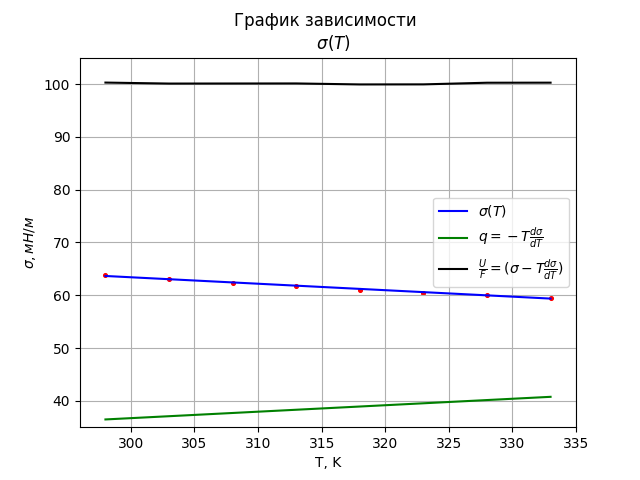
\includegraphics [scale=1]{surface_tension.png}}
\end{figure}

\item По МНК определяем коэффициент наклона прямой $\sigma (T)$: $k = \frac{d\sigma}{dT} = -0,122 \pm 0,003$ мН/м$\cdot$К
	\end{enumerate}

	\textbf{Обсуждение результатов: }\\
В данной работе мы определили двумя способами диаметр иголки, полученные значения совпадают в пределах погрешностей. Также мы двумя способами определили длину иголки, полученные значения также совпадают в пределах погрешностей. Полученный нами коэффициент поверхностного натяжения жидкости не совпадает с табличным в пределах погрешности ($\sigma = 73$ мН/м при T = 298 К)



	\textbf{Выводы: }\\ В ходе данной работы мы
измерили температурные зависимости коэффициента поверхностного
натяжения дистиллированной воды с использованием известного коэффициента
поверхностного натяжения спирта; 2) определили полную поверхностную энергию и
теплоту, необходимую для изотермического образования единицы поверхности жидкости
при различной температуре

	\end{document}